\clearpage
\sffamily
\added{
{\bfseries\color[rgb]{0.4,0.4,0.4} Manual for building a Parkour Technical
Challenge for Kid and Adult size}
\phantomsection
\addcontentsline{toc}{subsection}{Manual for building a Parkour Technical
Challenge for Kid and Adult size}

\bigskip

The parkour technical challenge is composed of piled platforms. 

The minimum height is 1/5th of the robot's height.
% NOTE: Maximal height should be Sweaty with 168cm
The main platform's height is 5 cm, and it has an area of 60x60 cm.
When the platforms are stacked,
they form a stack with resultant height of a multiple of 5cm.

This document provides two different options to build the piled platforms.

\bigskip

{\bfseries Materials}

\headlinebox

\begin{itemize}
\item 2 wooden platforms [dimensions 60 x 60 x 5 cm]
      (see Figure~\ref{fig:parkour-top-platform-with-hook-and-loop})
\item 3 squares of turf\footnote{Same turf used for games fields}
      [dimensions 60 x 60 cm] (2 square as backup)
\item Option 1:
      \begin{itemize}
      \item 28 L-shape wooden supports [dimensions 20x20x7 cm and height 5 cm]
            (see Figure 3)
      \item 48 wooden dowels\footnote{Having extra wooden dowels as spare is
              recommendable in case they break} [dimensions 6 mm x 40 mm]
      \end{itemize}
\item Option 2:
      \begin{itemize}
      \item 14 straight wooden supports [dimension around 40x7 cm and height 5
            cm] (see Figure 4)
      \item 12 wooden dowels\footnote{Having extra wooden dowels as spare is
              recommendable in case they break} [dimensions 6 mm x 40 mm]
      \end{itemize}
\item 4 hook-and-loop fasteners for one platform and the turf,
      for a total of 8 hook-and-loop fasteners
      (see Figures~\ref{fig:parkour-hook-and-loop} and
      \ref{fig:parkour-top-platform-with-hook-and-loop})
      \begin{itemize}
      \item 2 hook-and-loop fasteners [dimension around 30 x 7.5 cm]
      \item 2 hook-and-loop fasteners [dimension around 40 x 7.5 cm]
      \end{itemize}
\end{itemize}

\begin{figure}[htb]
  \begin{subfigure}{.45\textwidth}
    \centering
    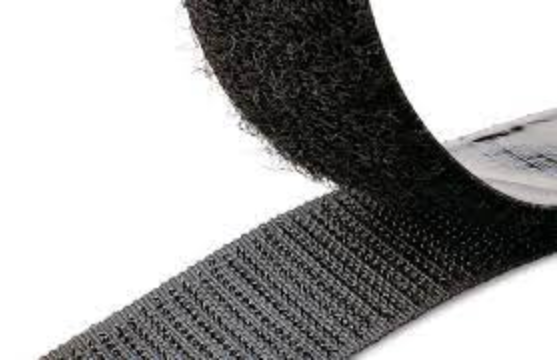
\includegraphics[width=\textwidth]{img/parkour/hook_and_loop}
    \caption{Hook-and-loop fasteners.}
    \label{fig:parkour-hook-and-loop}
  \end{subfigure}
  \hfill
  \begin{subfigure}{.45\textwidth}
    \centering
    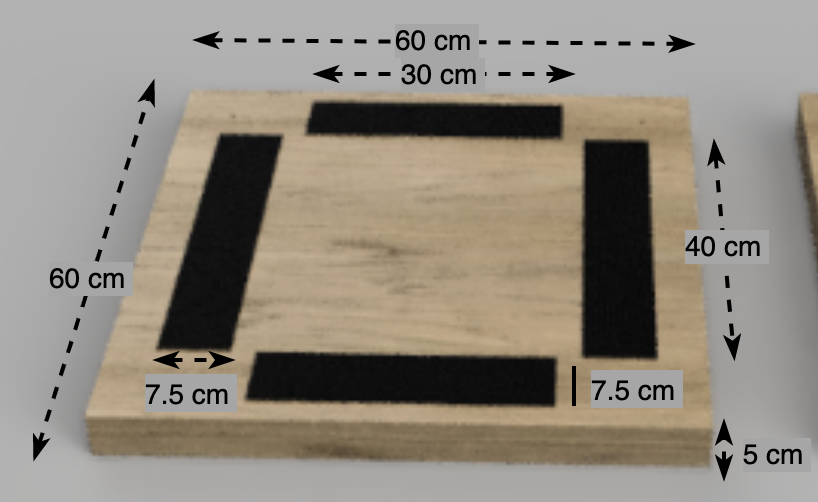
\includegraphics[width=\textwidth]{img/parkour/top_fasteners}
    \caption{Top platform with hook-and-loop fasteners.}
    \label{fig:parkour-top-platform-with-hook-and-loop}
  \end{subfigure}
  \caption{Usage of hook-and-loop fasteners for the Parkour platform.}
\end{figure}

\begin{figure}[htb]
  \begin{subfigure}{.45\textwidth}
    \centering
    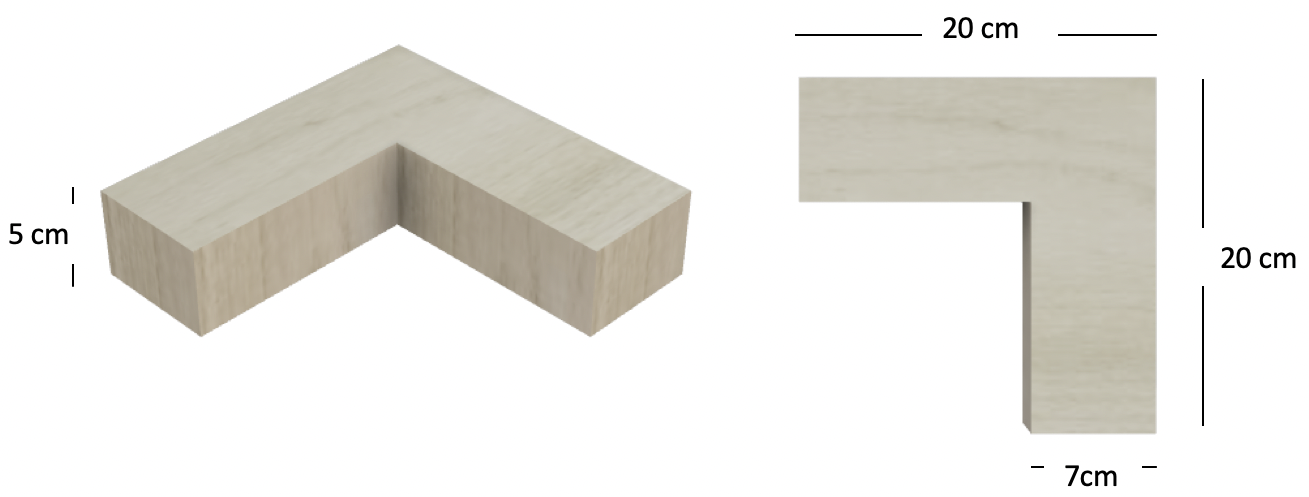
\includegraphics[width=\textwidth]{img/parkour/option1_support}
    \caption{L-shape wooden support.}
    \label{fig:parkour-option1-support}
  \end{subfigure}
  \hfill
  \begin{subfigure}{.45\textwidth}
    \centering
    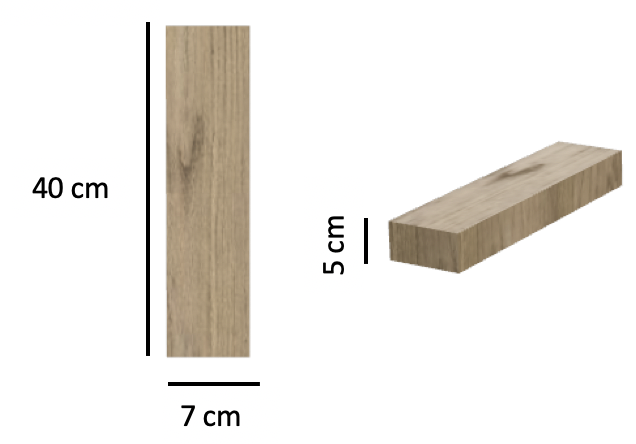
\includegraphics[width=\textwidth]{img/parkour/option2_support}
    \caption{Straight wooden support.}
    \label{fig:parkour-option2-support}
  \end{subfigure}
  \caption{Different support options for the Parkour platform.}
\end{figure}

\bigskip

{\bfseries Common instructions}

\headlinebox

The top of the top platform is covered with turf
(see Figure~\ref{fig:parkour-top-turf})
The turf is attachable and detachable using hook-and-loop fasteners
(double adhesive velcro tape - one side attached to the platform,
one side attached to the back of the turf piece). 

To increase the height of the platform,
add the 4 wooden dowels (see Figure~\ref{fig:parkour-wooden-dowels})
in the holes on the top surface of the platform and add the external supports.
Holes in the platform should be 2 cm deep.

\begin{figure}[htb]
  \begin{subfigure}{.45\textwidth}
    \centering
    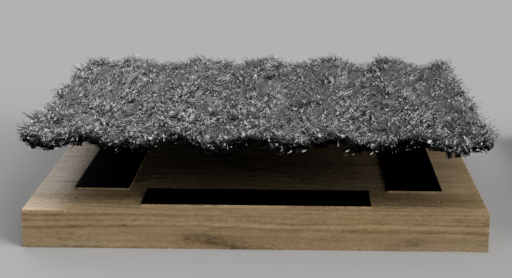
\includegraphics[width=\textwidth]{img/parkour/top_turf}
    \caption{Platform with turf on top.}
    \label{fig:parkour-top-turf}
  \end{subfigure}
  \hfill
  \begin{subfigure}{.45\textwidth}
    \centering
    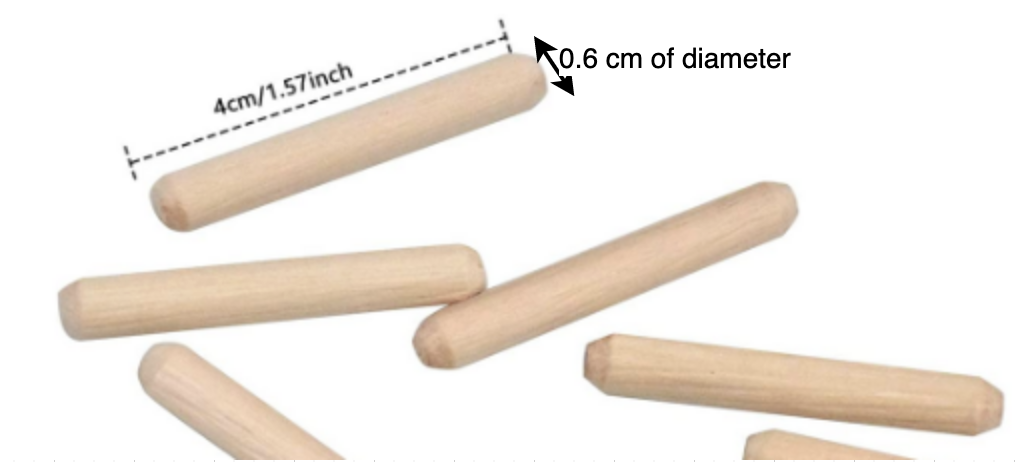
\includegraphics[width=\textwidth]{img/parkour/wooden_dowels}
    \caption{Wooden dowels.}
    \label{fig:parkour-wooden-dowels}
  \end{subfigure}
  \caption{Common assembly parts for both options.}
\end{figure}

\bigskip

{\bfseries Option 1: increase the height of the platform with L-shape wooden
           supports}

\headlinebox

4 L-shape wooden supports are fixed on the 4 corners of the lower platform to
increase the height (see Figure~\ref{fig:parkour-option1-lower}).
Each L-shape wooden support needs to fixed on the wooden platforms lower and
upper with the wooden dowels to be stable
(see Figure~\ref{fig:parkour-option1-full}). 

\begin{figure}[htb]
  \begin{subfigure}{.45\textwidth}
    \centering
    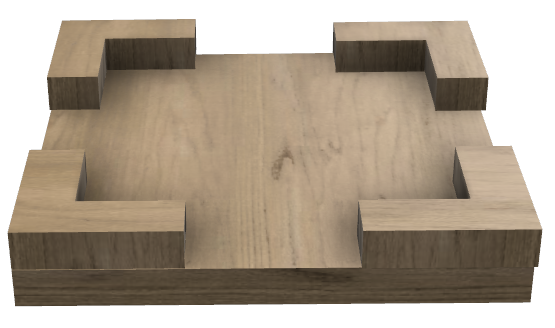
\includegraphics[width=\textwidth]{img/parkour/option1_lower}
    \caption{Lower platform with Option 1 L-shape wooden supports for increasing
             height.}
    \label{fig:parkour-option1-lower}
  \end{subfigure}
  \hfill
  \begin{subfigure}{.45\textwidth}
    \centering
    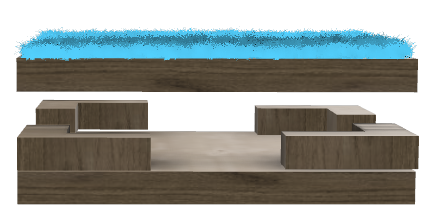
\includegraphics[width=\textwidth]{img/parkour/option1_full}
    \caption{Lower and upper platform with Option 1 L-shape wooden supports
             for increasing height.}
    \label{fig:parkour-option1-full}
  \end{subfigure}
  \caption{Option 1: using L-shape wooden supports.}
\end{figure}

\bigskip

{\bfseries Option 2: increase the height of the platform with straight wooden
           supports}

\headlinebox

2 wooden supports are fixed on two sides of the lower platform to increase the
height (see Figure~\ref{fig:parkour-option2-lower}).
Each wooden support needs to fixed on the wooden lower and top platforms with
the wooden dowels to be stable (see Figure~\ref {fig:parkour-option2-full}).

\begin{figure}[htb]
  \begin{subfigure}{.45\textwidth}
    \centering
    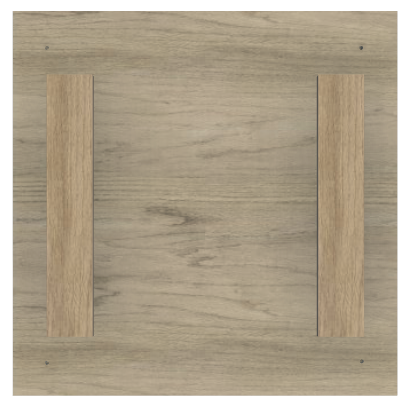
\includegraphics[width=\textwidth]{img/parkour/option2_lower}
    \caption{Lower platform with Option 2 straight wooden supports for increasing
             height.}
    \label{fig:parkour-option2-lower}
  \end{subfigure}
  \hfill
  \begin{subfigure}{.45\textwidth}
    \centering
    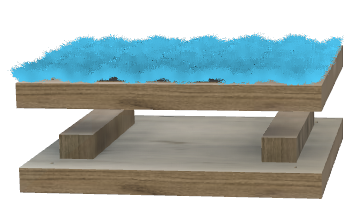
\includegraphics[width=\textwidth]{img/parkour/option2_full}
    \caption{Lower and upper platform with Option 2 straight wooden supports
             for increasing height.}
    \label{fig:parkour-option2-full}
  \end{subfigure}
  \caption{Option 2: using straight wooden supports.}
\end{figure}

}